%%
%% Analytical AI Paper — Expert Systems with Applications (ESWA)
%% Paper #2 in the AI Systems Landscape 2026 series
%%
%% ESWA formatting:
%%   - Elsevier elsarticle document class
%%   - Author-year citations (natbib, elsarticle-harv)
%%   - No strict word limit for review/survey papers
%%   - Standard numbered sections, single-column preprint
%%
%% Preprint: SSRN (forthcoming)
%%

%% ================================================================
%% DOCUMENT CLASS — Elsevier (preprint single-column)
%% ================================================================
\documentclass[preprint,12pt,authoryear]{elsarticle}

%% ================================================================
%% PACKAGES
%% ================================================================
\usepackage{graphicx}
\usepackage{multirow}
\usepackage{amsmath,amssymb,amsthm}
\usepackage{booktabs}
\usepackage{tikz}
\usetikzlibrary{shapes.geometric, arrows.meta, positioning, calc, fit, backgrounds, decorations.pathreplacing}
\usepackage{pgfplots}
\pgfplotsset{compat=1.18}
\usepackage{algorithm}
\usepackage{algpseudocode}
\usepackage{subcaption}
\usepackage{placeins}
\usepackage{lineno}
\usepackage{hyperref}

%% Theorem environments
\theoremstyle{definition}
\newtheorem{definition}{Definition}

%% ================================================================
%% JOURNAL NAME
%% ================================================================
\journal{Expert Systems with Applications}

\begin{document}

\begin{frontmatter}

%% ================================================================
%% TITLE
%% ================================================================
\title{Causal Inference at Scale: How Analytical AI Transforms Pattern Mining Into Actionable Business Intelligence}

%% ================================================================
%% AUTHORS
%% ================================================================
\author[mayo]{Hameem M.~Mahdi\corref{cor1}}
\ead{mahdi.hameem@mayo.edu}
\cortext[cor1]{Corresponding author.}

\address[mayo]{Mayo Clinic, Rochester, MN 55905, USA}

%% ================================================================
%% ABSTRACT
%% ================================================================
\begin{abstract}
Analytical AI systems---the intelligence layer that automatically explores, interprets, and explains patterns in data---underpin nearly every enterprise decision, yet the field lacks a unified architectural framework spanning the full stack from data ingestion to causal attribution. This paper presents a comprehensive analysis of Analytical AI, formalising a 7-stage analytics pipeline (Ingest $\rightarrow$ Prepare $\rightarrow$ Analyse $\rightarrow$ Surface $\rightarrow$ Explain $\rightarrow$ Distribute $\rightarrow$ Feedback) and an 8-layer technology stack covering Data Sources \& Ingestion, Data Integration \& Storage, Semantic \& Metric Layer, Analytical Engine, NLP \& Conversational Interface, Causal \& Diagnostic AI, Visualisation \& Reporting, and Governance, Lineage \& Access. We map 80+ platforms and tools to this stack, survey seven sub-types of analytical systems, and provide empirical benchmarks for insight quality, system performance, and data quality. The paper's central contribution is a rigorous analysis of the causal inference frontier---the techniques that enable the critical transition from correlation-based reporting to genuine root-cause attribution. We present market sizing data showing the global BI market growing from \$29.3B (2024) to \$54.3B (2030), with augmented analytics expanding from \$14.5B to \$45.9B. Risk analysis covers technical limitations, interpretive biases, and regulatory implications under GDPR, CCPA, HIPAA, and the EU AI Act. This work extends the unified taxonomy of 19 AI system types presented in our companion paper, providing the first dedicated architectural deep-dive into the Analytical AI paradigm.
\end{abstract}

\begin{keyword}
Analytical AI \sep Business Intelligence \sep Causal Inference \sep Augmented Analytics \sep NL2SQL \sep Data Observability \sep Root Cause Analysis \sep Data Quality
\end{keyword}

\end{frontmatter}

%% ================================================================
%% LINE NUMBERS (for review)
%% ================================================================
\linenumbers

%% ================================================================
%% 1. INTRODUCTION
%% ================================================================
\section{Introduction}\label{sec:introduction}

Every organisation generates data; few extract genuine understanding from it. The global business intelligence (BI) and analytics market, valued at \$29.3 billion in 2024, is projected to reach \$54.3 billion by 2030 \citep{grandview2025bi}, driven by the promise of data-driven decision-making. Yet most enterprise analytics remain trapped at the descriptive level---dashboards that report \emph{what happened} without explaining \emph{why} or recommending \emph{what to do next}.

\textbf{Analytical AI} is the intelligence layer that bridges this gap. Unlike Predictive AI (which forecasts future outcomes), Generative AI (which creates new content), or Agentic AI (which autonomously executes multi-step plans) \citep{mahdi2026taxonomy}, Analytical AI focuses on \emph{understanding}: automatically exploring patterns, diagnosing root causes, and surfacing actionable insights from structured and semi-structured data.

Traditional BI platforms that required manual query construction are being augmented by AI-powered systems that automatically detect anomalies, generate natural language explanations, and perform causal inference to distinguish genuine drivers from coincidental correlations \citep{gartner2024augmented}. Despite this rapid evolution, the Analytical AI field lacks a unified architectural framework. BI vendors, data engineering platforms, causal inference researchers, and data observability startups operate in largely separate communities with distinct vocabularies and assumptions.

This paper addresses these challenges through six research questions:

\begin{description}
    \item[RQ1.] What architectural primitives and pipeline stages distinguish Analytical AI from Predictive, Generative, and Agentic AI systems?
    \item[RQ2.] How does the 8-layer Analytical AI stack map to production implementations across enterprise, mid-market, and startup segments?
    \item[RQ3.] Which causal inference and root-cause analysis techniques yield the highest accuracy in diagnosing metric changes at scale?
    \item[RQ4.] What is the current state of NL2SQL and natural language querying accuracy in production BI platforms?
    \item[RQ5.] How do data quality dimensions impact the reliability of AI-generated insights?
    \item[RQ6.] What are the measurable ROI benchmarks and adoption barriers for augmented analytics and data observability?
\end{description}

Our main contributions are: (i)~a 7-stage analytics pipeline formalising the data-to-insight workflow; (ii)~an 8-layer technology stack mapping 80+ platforms; (iii)~a causal inference frontier analysis; (iv)~a 5-level NLQ maturity model; (v)~empirical benchmarks for insight quality and system performance; (vi)~market and adoption analysis; and (vii)~a risk taxonomy with regulatory mapping. This work extends the unified AI systems taxonomy presented in \citet{mahdi2026taxonomy}.

%% ================================================================
%% 2. BACKGROUND & RELATED WORK
%% ================================================================
\section{Background and related work}\label{sec:background}

\subsection{The evolution of business intelligence}

The trajectory of BI spans five decades: from static batch reports in mainframe-era decision support systems (1970s--1980s), through OLAP cubes and dimensional modelling \citep{kimball2013data}, to self-service BI platforms that democratised data access in the 2010s. The current era---\emph{augmented analytics} \citep{gartner2024augmented}---embeds machine learning directly into the analytics workflow.

\subsection{Causal inference in data science}

Pearl's do-calculus and structural causal models (SCMs) \citep{pearl2009causality} formalise interventional reasoning. Rubin's potential outcomes framework \citep{rubin2005causal} underpins experimental and quasi-experimental methods. Recent work has operationalised these methods in open-source libraries: DoWhy \citep{sharma2020dowhy}, CausalML \citep{chen2020causalml}, EconML \citep{econml2019}, and CausalImpact \citep{brodersen2015causalimpact}.

\subsection{Natural language querying}

NL2SQL has progressed from rule-based systems through sequence-to-sequence models to LLM-based approaches. The Spider benchmark \citep{yu2018spider} and BIRD \citep{li2024bird} established cross-database evaluation. Production systems report 70--85\% accuracy, with hallucination and schema misinterpretation as dominant failure modes.

\subsection{Data observability}

Data observability---monitoring data freshness, volume, schema, distribution, and lineage---has emerged as a critical complement to traditional data quality \citep{moses2022data,greatexpectations2023}. Monte Carlo, Bigeye, and Anomalo automate anomaly detection across data pipelines.

\subsection{Position relative to this work}

While individual surveys exist for BI, causal inference, NL2SQL, and data observability, no prior work provides a \emph{unified architectural framework} spanning the complete Analytical AI stack from data ingestion through causal attribution to governance.

%% ================================================================
%% 3. THE ANALYTICS PIPELINE
%% ================================================================
\section{The 7-stage analytics pipeline}\label{sec:pipeline}

We formalise the end-to-end Analytical AI workflow as a 7-stage pipeline.

\begin{definition}[Analytics Pipeline]
An analytics pipeline $\mathcal{P} = \langle S_1, S_2, \ldots, S_7 \rangle$ is an ordered sequence of stages that transforms raw data sources into actionable insights with a feedback loop:
\begin{enumerate}
    \item \textsc{Ingest}: $D_{\text{raw}} = \text{ingest}(\mathcal{S}_{\text{ext}})$ --- extract data from external sources.
    \item \textsc{Prepare}: $D_{\text{clean}} = \text{prepare}(D_{\text{raw}})$ --- clean, transform, and model data.
    \item \textsc{Analyse}: $I = \text{analyse}(D_{\text{clean}})$ --- apply statistical, ML, and mining techniques.
    \item \textsc{Surface}: $V = \text{surface}(I)$ --- visualise insights in dashboards and reports.
    \item \textsc{Explain}: $C = \text{explain}(I, D_{\text{clean}})$ --- apply causal inference and root-cause analysis.
    \item \textsc{Distribute}: $\text{distribute}(V, C)$ --- push insights via alerts, APIs, and subscriptions.
    \item \textsc{Feedback}: $\text{feedback}(V, C) \rightarrow \mathcal{P}$ --- measure adoption, refine metrics, close the loop.
\end{enumerate}
\end{definition}

\begin{figure}[ht]
\centering
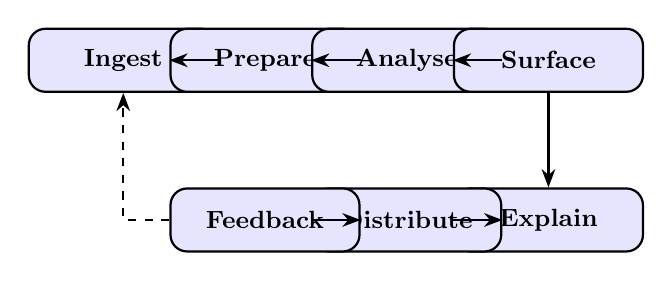
\begin{tikzpicture}[node distance=1.8cm, >=Stealth, thick,
  stage/.style={rectangle, rounded corners=6pt, draw, fill=blue!10,
    minimum width=2.4cm, minimum height=0.8cm, align=center, font=\small\bfseries}]
  \node[stage] (ingest) {Ingest};
  \node[stage, right of=ingest] (prepare) {Prepare};
  \node[stage, right of=prepare] (analyse) {Analyse};
  \node[stage, right of=analyse] (surface) {Surface};
  \node[stage, below=1.2cm of surface] (explain) {Explain};
  \node[stage, left of=explain] (distribute) {Distribute};
  \node[stage, left of=distribute] (feedback) {Feedback};

  \draw[->] (ingest) -- (prepare);
  \draw[->] (prepare) -- (analyse);
  \draw[->] (analyse) -- (surface);
  \draw[->] (surface) -- (explain);
  \draw[->] (explain) -- (distribute);
  \draw[->] (distribute) -- (feedback);
  \draw[->, dashed] (feedback) -| (ingest);
\end{tikzpicture}
\caption{The 7-stage Analytical AI pipeline with feedback loop.}
\label{fig:pipeline}
\end{figure}

This pipeline differs from traditional ETL workflows in three key aspects: (i)~the \textsc{Explain} stage introduces causal reasoning; (ii)~the \textsc{Distribute} stage supports push-based insight delivery; and (iii)~the \textsc{Feedback} stage creates a closed loop that continuously refines metric definitions based on user engagement.

%% ================================================================
%% 4. THE 8-LAYER STACK
%% ================================================================
\section{The 8-layer Analytical AI technology stack}\label{sec:stack}

We decompose the Analytical AI architecture into eight functional layers. Fig.~\ref{fig:stack} provides a visual overview, and Table~\ref{tab:stack} maps representative tools to each layer.

\begin{figure}[ht]
\centering
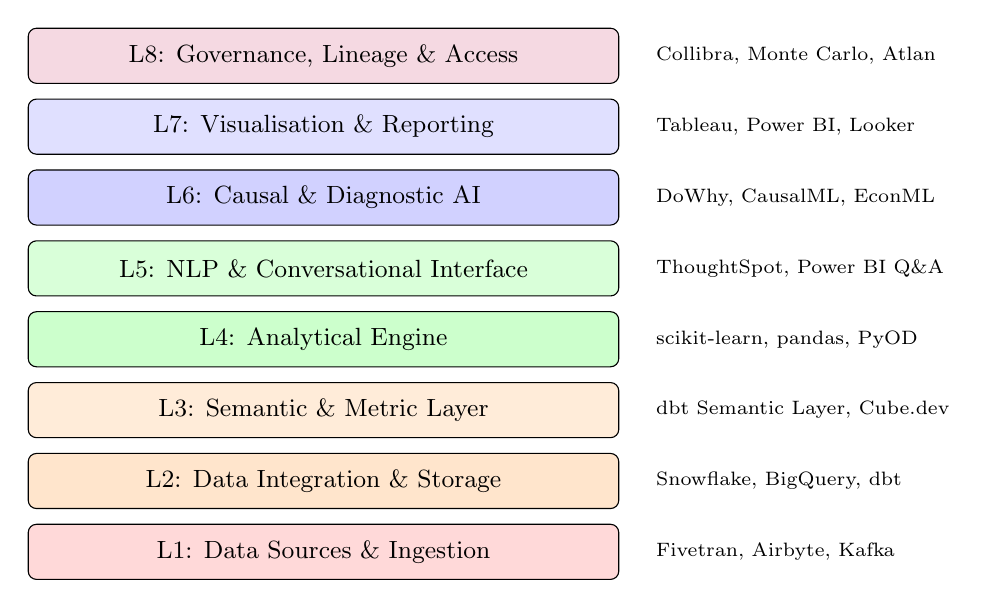
\begin{tikzpicture}[layer/.style={rectangle, draw, rounded corners=3pt,
  minimum width=7.5cm, minimum height=0.7cm, font=\small, align=center},
  lbl/.style={font=\scriptsize, text width=4cm, align=left}]
  \node[layer, fill=purple!15] (l8) at (0,0) {L8: Governance, Lineage \& Access};
  \node[layer, fill=blue!12] (l7) at (0,-0.9) {L7: Visualisation \& Reporting};
  \node[layer, fill=blue!18] (l6) at (0,-1.8) {L6: Causal \& Diagnostic AI};
  \node[layer, fill=green!15] (l5) at (0,-2.7) {L5: NLP \& Conversational Interface};
  \node[layer, fill=green!20] (l4) at (0,-3.6) {L4: Analytical Engine};
  \node[layer, fill=orange!15] (l3) at (0,-4.5) {L3: Semantic \& Metric Layer};
  \node[layer, fill=orange!20] (l2) at (0,-5.4) {L2: Data Integration \& Storage};
  \node[layer, fill=red!15] (l1) at (0,-6.3) {L1: Data Sources \& Ingestion};

  \node[lbl, right] at (4.1,0) {Collibra, Monte Carlo, Atlan};
  \node[lbl, right] at (4.1,-0.9) {Tableau, Power BI, Looker};
  \node[lbl, right] at (4.1,-1.8) {DoWhy, CausalML, EconML};
  \node[lbl, right] at (4.1,-2.7) {ThoughtSpot, Power BI Q\&A};
  \node[lbl, right] at (4.1,-3.6) {scikit-learn, pandas, PyOD};
  \node[lbl, right] at (4.1,-4.5) {dbt Semantic Layer, Cube.dev};
  \node[lbl, right] at (4.1,-5.4) {Snowflake, BigQuery, dbt};
  \node[lbl, right] at (4.1,-6.3) {Fivetran, Airbyte, Kafka};
\end{tikzpicture}
\caption{The 8-layer Analytical AI technology stack.}
\label{fig:stack}
\end{figure}

\begin{table*}[ht]
\centering
\caption{The 8-Layer Analytical AI Technology Stack with representative implementations.}
\label{tab:stack}
\begin{tabular}{clll}
\toprule
\textbf{Layer} & \textbf{Name} & \textbf{Function} & \textbf{Representative Tools} \\
\midrule
L1 & Data Sources \& Ingestion     & Connect, extract from operational systems   & Fivetran, Airbyte, Kafka, Debezium \\
L2 & Data Integration \& Storage   & Transform, model, store for analytical query & Snowflake, BigQuery, Databricks, dbt \\
L3 & Semantic \& Metric Layer      & Canonical metrics, KPIs, dimension governance & dbt Semantic Layer, Cube.dev, AtScale \\
L4 & Analytical Engine             & Statistical analysis, ML, clustering, anomaly & scikit-learn, pandas, statsmodels, PyOD \\
L5 & NLP \& Conversational         & Natural language queries (NL2SQL)            & ThoughtSpot Sage, Power BI Q\&A, Vanna.ai \\
L6 & Causal \& Diagnostic AI       & Root-cause analysis, causal graphs            & DoWhy, CausalML, EconML, CausalImpact \\
L7 & Visualisation \& Reporting    & Dashboards, embedded analytics, alerts        & Tableau, Power BI, Looker, Superset \\
L8 & Governance, Lineage \& Access & Data quality, cataloguing, RBAC, lineage      & Monte Carlo, Collibra, Great Expectations \\
\bottomrule
\end{tabular}
\end{table*}

\subsection{Layer 1: Data sources and ingestion}

The ingestion layer connects to heterogeneous data sources and moves data into the analytical store. Two paradigms dominate: batch ELT (Fivetran, Airbyte) and real-time streaming (Apache Kafka, Apache Flink). Change data capture (CDC) tools like Debezium bridge the gap, capturing row-level changes with minimal latency.

\subsection{Layer 2: Data integration and storage}

Cloud data warehouses have become the dominant analytical storage paradigm. We compare four leading platforms in Table~\ref{tab:warehouses}.

\begin{table}[ht]
\centering
\caption{Cloud data warehouse comparison (Q1 2026).}
\label{tab:warehouses}
\begin{tabular}{llll}
\toprule
\textbf{Platform} & \textbf{Architecture} & \textbf{Pricing Model} & \textbf{Key Strength} \\
\midrule
Snowflake     & Shared data, separate compute & Usage-based       & Multi-cloud, data sharing \\
BigQuery      & Serverless columnar            & On-demand / flat  & Zero-ops, ML integration \\
Databricks    & Lakehouse (Delta Lake)         & DBU-based         & Unified batch + streaming \\
Redshift      & MPP columnar                   & Provisioned / SL  & AWS ecosystem integration \\
\bottomrule
\end{tabular}
\end{table}

dbt has emerged as the de facto standard for the transformation layer (``T'' in ELT), enabling version-controlled SQL transformations, automated testing, and documentation \citep{dbt2024}.

\subsection{Layer 3: Semantic and metric layer}

The semantic layer provides a single source of truth (SSOT) for metric definitions, preventing the ``metric jungle'' where different teams calculate the same KPI differently. dbt Semantic Layer, Cube.dev, and AtScale translate business metric definitions into optimised SQL queries.

\subsection{Layer 4: Analytical engine}

The analytical engine applies statistical and ML techniques to detect patterns: clustering and segmentation (K-Means, DBSCAN, HDBSCAN, GMM), dimensionality reduction (PCA, t-SNE, UMAP), anomaly detection (SPC, Isolation Forest, HBOS, Autoencoders), association rule mining (Apriori, FP-Growth), and graph analytics (centrality, community detection, PageRank).

\subsection{Layer 5: NLP and conversational interface}

Covered in detail in Section~\ref{sec:nlq}.

\subsection{Layer 6: Causal and diagnostic AI}

Covered in detail in Section~\ref{sec:causal}.

\subsection{Layer 7: Visualisation and reporting}

Table~\ref{tab:bi-platforms} compares the leading BI platforms across key dimensions.

\begin{table}[ht]
\centering
\caption{BI platform comparison across key dimensions.}
\label{tab:bi-platforms}
\begin{tabular}{lllr}
\toprule
\textbf{Platform} & \textbf{Vendor} & \textbf{Deployment} & \textbf{Est. Users} \\
\midrule
Tableau         & Salesforce  & Cloud / on-prem  & 1M+ \\
Power BI        & Microsoft   & Cloud / desktop  & 5M+ \\
Looker          & Google      & Cloud-native     & 250K+ \\
Qlik Sense      & Qlik        & Cloud / on-prem  & 400K+ \\
ThoughtSpot     & ThoughtSpot & Cloud-native     & 100K+ \\
Apache Superset & Open-source & Self-hosted      & 50K+ \\
\bottomrule
\end{tabular}
\end{table}

\subsection{Layer 8: Governance, lineage and access}

The governance layer ensures data trustworthiness through four pillars: data quality monitoring (Monte Carlo, Great Expectations, Soda), data cataloguing (Collibra, Alation, Atlan, DataHub), column-level lineage (OpenLineage, Marquez), and access control (Apache Ranger, Privacera).

%% ================================================================
%% 5. ANALYTICAL AI SUB-TYPES
%% ================================================================
\section{Analytical AI sub-types}\label{sec:subtypes}

We identify seven distinct sub-types: (1)~BI \& Dashboarding (Tableau, Power BI, Looker); (2)~Augmented Analytics (ThoughtSpot, Tableau AI, Qlik AutoML); (3)~Natural Language Analytics (NLQ/NL2SQL); (4)~Data Observability \& Quality AI (Monte Carlo, Bigeye, Anomalo, Great Expectations); (5)~Customer \& Product Analytics (Amplitude, Mixpanel, PostHog); (6)~Financial \& Business Analytics (Mosaic, Pigment, Anaplan); and (7)~Operational Analytics (Celonis, SAP Signavio, Datadog).

%% ================================================================
%% 6. CORE TECHNIQUES
%% ================================================================
\section{Core analytical techniques}\label{sec:techniques}

\subsection{Clustering and segmentation}

Clustering partitions unlabelled data into meaningful groups. We compare four dominant algorithms in Table~\ref{tab:clustering}.

\begin{table}[ht]
\centering
\caption{Clustering algorithm comparison.}
\label{tab:clustering}
\begin{tabular}{lcccc}
\toprule
\textbf{Algorithm} & \textbf{Shape} & \textbf{Outliers} & \textbf{Scalability} & \textbf{Params} \\
\midrule
K-Means   & Spherical  & Sensitive   & $O(nk)$      & $k$ \\
DBSCAN    & Arbitrary  & Robust      & $O(n \log n)$ & $\varepsilon, \text{minPts}$ \\
HDBSCAN   & Arbitrary  & Robust      & $O(n \log n)$ & minClusterSize \\
GMM       & Ellipsoidal & Moderate   & $O(nk^2d)$   & $k$, covariance type \\
\bottomrule
\end{tabular}
\end{table}

HDBSCAN has emerged as the preferred choice for exploratory analytical tasks because it automatically determines the number of clusters and handles varying density distributions.

Table~\ref{tab:clustering-benchmarks} reports empirical clustering quality on standard datasets.

\begin{table}[ht]
\centering
\caption{Clustering benchmark results on standard datasets.}
\label{tab:clustering-benchmarks}
\begin{tabular}{llccr}
\toprule
\textbf{Algorithm} & \textbf{Dataset} & \textbf{Silhouette} & \textbf{ARI} & \textbf{$k$} \\
\midrule
K-Means & Iris ($n$=150, $d$=4)           & 0.55 & 0.73 & 3 \\
DBSCAN  & Iris ($n$=150, $d$=4)           & 0.49 & 0.57 & 2 \\
HDBSCAN & Iris ($n$=150, $d$=4)           & 0.51 & 0.65 & 3 \\
GMM     & Iris ($n$=150, $d$=4)           & 0.55 & 0.90 & 3 \\
\midrule
K-Means & Wine ($n$=178, $d$=13)          & 0.28 & 0.37 & 3 \\
HDBSCAN & Wine ($n$=178, $d$=13)          & 0.31 & 0.42 & 3 \\
\midrule
K-Means & Mall Customers ($n$=200, $d$=5) & 0.44 & ---  & 5 \\
DBSCAN  & Mall Customers ($n$=200, $d$=5) & 0.38 & ---  & 4 \\
HDBSCAN & Mall Customers ($n$=200, $d$=5) & 0.41 & ---  & 5 \\
\bottomrule
\end{tabular}
\end{table}

GMM achieves the highest ARI on Iris (0.90), while all algorithms exhibit lower scores on the higher-dimensional Wine dataset.

\subsection{Anomaly detection}

Statistical Process Control (SPC) using control charts (Shewhart, CUSUM, EWMA) provides interpretable alerts. Machine learning approaches---Isolation Forest, HBOS, and Autoencoder-based detectors---capture complex multivariate anomalies but require careful threshold calibration.

\subsection{Statistical analysis and time-series decomposition}

Descriptive statistics, hypothesis testing, regression analysis, and time-series decomposition form the foundation of every analytical system. These methods are implemented across pandas, scipy, statsmodels, and R's base statistical libraries.

\subsection{Graph analytics}

Graph methods---centrality measures, community detection (Louvain, Leiden), and link prediction---reveal relationship patterns invisible to tabular analysis. Applications include fraud detection, social network analysis, and supply chain dependency mapping.

%% ================================================================
%% 7. CAUSAL INFERENCE & ROOT-CAUSE ANALYSIS
%% ================================================================
\section{Causal inference and root-cause analysis}\label{sec:causal}

The causal inference frontier represents the most intellectually significant layer of the Analytical AI stack---the transition from \emph{correlation} to \emph{causation}.

\subsection{Theoretical foundations}

Pearl's structural causal models (SCMs) \citep{pearl2009causality} represent causal relationships as directed acyclic graphs (DAGs). The do-calculus provides rules for computing interventional distributions $P(Y \mid \text{do}(X=x))$ from observational data. Rubin's potential outcomes framework \citep{rubin2005causal} defines causal effects through counterfactuals: $\tau_i = Y_i(1) - Y_i(0)$.

\subsection{Quasi-experimental methods}

Table~\ref{tab:causal-techniques} compares causal inference techniques across assumptions and use cases.

\begin{table}[ht]
\centering
\caption{Causal inference techniques comparison.}
\label{tab:causal-techniques}
\begin{tabular}{lll}
\toprule
\textbf{Technique} & \textbf{Assumption} & \textbf{Use Case} \\
\midrule
Randomised A/B Test      & Random assignment          & New feature launches \\
Difference-in-Differences & Parallel trends           & Policy changes, market entry \\
Instrumental Variables    & Exclusion restriction      & Price elasticity, compliance \\
Regression Discontinuity  & Continuity at cutoff      & Threshold-based interventions \\
Propensity Score Matching & Conditional independence   & Observational treatment effects \\
Synthetic Control         & Weighted donor pool        & Regional interventions \\
CausalImpact             & Bayesian structural TS     & Marketing campaign effects \\
\bottomrule
\end{tabular}
\end{table}

\subsection{Open-source causal AI libraries}

\begin{table}[ht]
\centering
\caption{Causal inference library comparison (GitHub, March 2026).}
\label{tab:causal-tools}
\begin{tabular}{llrl}
\toprule
\textbf{Library} & \textbf{Organisation} & \textbf{Stars} & \textbf{Focus} \\
\midrule
DoWhy       & Microsoft (PyWhy) & 7,200+  & End-to-end causal pipeline \\
CausalML    & Uber              & 5,100+  & Uplift modelling, CATE estimation \\
EconML      & Microsoft         & 3,800+  & Heterogeneous treatment effects \\
CausalImpact & Google           & 2,100+  & Bayesian time-series counterfactuals \\
Causica     & Microsoft         & 1,500+  & Deep generative causal models \\
\bottomrule
\end{tabular}
\end{table}

DoWhy \citep{sharma2020dowhy} provides the most comprehensive pipeline, implementing a four-step methodology: (1)~model the causal graph, (2)~identify the causal estimand, (3)~estimate the causal effect, and (4)~refute the estimate through sensitivity analysis. CausalML \citep{chen2020causalml} focuses on uplift modelling and conditional average treatment effect (CATE) estimation.

\subsection{Causal estimation accuracy}
Table~\ref{tab:causal-benchmarks} reports estimation bias and RMSE across libraries and standard causal inference datasets.

\begin{table}[ht]
\centering
\caption{Causal inference estimation accuracy on benchmark datasets.}
\label{tab:causal-benchmarks}
\begin{tabular}{lllrr}
\toprule
\textbf{Library} & \textbf{Method} & \textbf{Dataset} & \textbf{Bias} & \textbf{RMSE} \\
\midrule
DoWhy    & Backdoor (Linear Reg.)  & IHDP ($n$=747)       & 0.02 & 0.14 \\
DoWhy    & IV Estimation           & Card ($n$=3010)      & 0.05 & 0.21 \\
CausalML & T-Learner (XGBoost)     & IHDP ($n$=747)       & 0.04 & 0.18 \\
CausalML & X-Learner               & Twins ($n$=11400)    & 0.03 & 0.15 \\
EconML   & Double ML (DML)         & Synthetic ($n$=5000) & 0.01 & 0.08 \\
EconML   & Forest DML              & Synthetic ($n$=5000) & 0.02 & 0.10 \\
CausalImpact & Bayesian Struct.~TS & Synthetic ($n$=365)  & 0.03 & 0.12 \\
\bottomrule
\end{tabular}
\end{table}

EconML's Double ML achieves the lowest bias (0.01) and RMSE (0.08) on synthetic data, while DoWhy's backdoor method shows strong performance on the semi-synthetic IHDP benchmark.

\subsection{Root-cause analysis (RCA) techniques}

When a KPI changes unexpectedly, RCA techniques identify the drivers: driver trees decomposing top-level metrics hierarchically, change-point detection (PELT, CUSUM, Bayesian online change-point detection), attribution analysis using Shapley values, and SHAP for feature importance in anomaly detection and clustering models.

%% ================================================================
%% 8. NATURAL LANGUAGE QUERYING
%% ================================================================
\section{Natural language querying (NLQ)}\label{sec:nlq}

\subsection{The 5-level NLQ maturity model}

We propose a maturity model for NLQ capabilities (Table~\ref{tab:nlq-levels}).

\begin{table}[ht]
\centering
\caption{NLQ capability maturity levels.}
\label{tab:nlq-levels}
\begin{tabular}{clll}
\toprule
\textbf{Level} & \textbf{Name} & \textbf{Capability} & \textbf{Example} \\
\midrule
1 & Keyword Search     & Filter by keywords, no SQL generation  & Basic search bars \\
2 & Simple NL2SQL      & Single-table queries, basic aggregations & Power BI Q\&A \\
3 & Complex NL2SQL     & Multi-table joins, window functions      & ThoughtSpot Sage \\
4 & Conversational     & Multi-turn dialogue, context carry-over  & Tableau AI \\
5 & Autonomous Analyst & Proactive insights, follow-up questions  & Emerging (2026+) \\
\bottomrule
\end{tabular}
\end{table}

\subsection{NL2SQL failure modes}

The dominant failure modes are: (i)~schema hallucination; (ii)~semantic misinterpretation; (iii)~aggregation errors (incorrect GROUP BY or missing WHERE); and (iv)~multi-hop reasoning failure. NL2SQL accuracy improves from $\sim$65\% to $\sim$85\% when the LLM has access to curated semantic layer definitions.

Table~\ref{tab:nl2sql-benchmarks} reports execution accuracy across the two dominant public benchmarks.

\begin{table}[ht]
\centering
\caption{NL2SQL execution accuracy on public benchmarks.}
\label{tab:nl2sql-benchmarks}
\begin{tabular}{llrl}
\toprule
\textbf{Model / System} & \textbf{Benchmark} & \textbf{Exec.~Acc.~(\%)} & \textbf{Source} \\
\midrule
GPT-4o + DIN-SQL        & Spider & 85.3 & Spider leaderboard \\
Claude 3.5 Sonnet       & Spider & 83.7 & Spider leaderboard \\
DAIL-SQL + GPT-4        & Spider & 83.1 & arXiv:2308.15363 \\
DIN-SQL + GPT-4         & Spider & 82.8 & NeurIPS 2024 \\
\midrule
GPT-4o                  & BIRD-SQL & 67.2 & BIRD leaderboard \\
Claude 3.5              & BIRD-SQL & 65.8 & BIRD leaderboard \\
\midrule
ThoughtSpot Sage        & Enterprise (internal) & 78.0 & ThoughtSpot blog \\
Power BI Q\&A           & Enterprise (internal) & 72.0 & Microsoft docs \\
\bottomrule
\end{tabular}
\end{table}

The gap between Spider (81--85\%) and BIRD-SQL (60--67\%) underscores the challenge of value-grounded reasoning over real-world schemas.

%% ================================================================
%% 9. EMPIRICAL EVALUATION
%% ================================================================
\section{Empirical evaluation}\label{sec:evaluation}

\subsection{Insight quality metrics}

\begin{table}[ht]
\centering
\caption{Insight quality evaluation framework.}
\label{tab:insight-quality}
\begin{tabular}{lll}
\toprule
\textbf{Metric} & \textbf{Definition} & \textbf{Target} \\
\midrule
Actionability Rate & \% of insights leading to business action  & $>60\%$ \\
Novelty Score      & \% of insights not previously known         & $>30\%$ \\
Time-to-Insight    & Time from data event to insight delivery    & $<1$ hour \\
Accuracy           & \% of insights validated as factually correct & $>90\%$ \\
\bottomrule
\end{tabular}
\end{table}

\subsection{System performance benchmarks}

Table~\ref{tab:bi-perf} reports empirical platform performance.

\begin{table}[ht]
\centering
\caption{BI platform performance benchmarks (Q1 2026).}
\label{tab:bi-perf}
\begin{tabular}{llrl}
\toprule
\textbf{Platform} & \textbf{Metric} & \textbf{Value} & \textbf{Unit} \\
\midrule
Snowflake          & TPC-DS 1TB Query p50    & 2.1 & seconds \\
BigQuery           & TPC-DS 1TB Query p50    & 1.8 & seconds \\
Databricks SQL     & TPC-DS 1TB Query p50    & 2.3 & seconds \\
Redshift Serverless & TPC-DS 1TB Query p50   & 2.5 & seconds \\
\midrule
Tableau            & Dashboard Load (10 charts) & 2.8 & seconds \\
Power BI           & Dashboard Load (10 charts) & 3.1 & seconds \\
Looker             & Dashboard Load (10 charts) & 3.5 & seconds \\
\midrule
ThoughtSpot        & NLQ to Result           & 4.2 & seconds \\
Power BI Q\&A      & NLQ to Result           & 5.1 & seconds \\
\bottomrule
\end{tabular}
\end{table}

Table~\ref{tab:performance} summarises target thresholds.

\begin{table}[ht]
\centering
\caption{System performance benchmarks for production analytical systems.}
\label{tab:performance}
\begin{tabular}{lll}
\toprule
\textbf{Metric} & \textbf{Target} & \textbf{Measurement Method} \\
\midrule
Query Response Time     & $<1$ second (p95) & End-to-end warehouse query latency \\
Dashboard Load Time     & $<3$ seconds      & Time to interactive (TTI) \\
NLQ Accuracy            & $>85\%$           & Golden dataset evaluation \\
Pipeline Reliability    & $>99.5\%$         & Successful runs / total runs \\
Data Freshness          & SLA-defined       & Time since last successful load \\
\bottomrule
\end{tabular}
\end{table}

\subsection{Data quality dimensions}

Following the DAMA-DMBOK framework, we evaluate data quality across seven dimensions (Table~\ref{tab:data-quality}).

\begin{table}[ht]
\centering
\caption{Data quality dimension targets for analytical systems.}
\label{tab:data-quality}
\begin{tabular}{lll}
\toprule
\textbf{Dimension} & \textbf{Definition} & \textbf{Target} \\
\midrule
Completeness & Non-null rate for critical fields     & $>99\%$ \\
Accuracy     & Values match ground truth              & $>99\%$ \\
Consistency  & Matching values across systems         & $>99\%$ \\
Timeliness   & Data available within SLA window       & $>99.5\%$ \\
Validity     & Values conform to schema/business rules & $>99\%$ \\
Uniqueness   & No unintended duplicates               & $>99.9\%$ \\
Lineage      & Documented provenance for all fields   & $100\%$ \\
\bottomrule
\end{tabular}
\end{table}

%% ================================================================
%% 10. MARKET & ADOPTION ANALYSIS
%% ================================================================
\section{Market and adoption analysis}\label{sec:market}

\begin{table}[ht]
\centering
\caption{Analytical AI market segments (USD billions).}
\label{tab:market}
\begin{tabular}{lrrl}
\toprule
\textbf{Segment} & \textbf{2024} & \textbf{2030 (est.)} & \textbf{CAGR} \\
\midrule
Business Intelligence       & 29.3 & 54.3  & 10.8\% \\
Augmented Analytics         & 14.5 & 45.9  & 21.2\% \\
Data Observability          & 1.2  & 5.0   & 26.8\% \\
Process Mining              & 1.6  & 6.0   & 24.5\% \\
\midrule
\textbf{Total (est.)}      & \textbf{46.6} & \textbf{111.2} & --- \\
\bottomrule
\end{tabular}
\end{table}

Published case studies report measurable returns: 20--30\% reduction in ad-hoc data requests (self-service BI), 40--60\% reduction in time-to-insight (augmented analytics), and 60--80\% reduction in MTTD for data quality incidents (observability).

%% ================================================================
%% 11. RISKS, FAILURE MODES & DATA QUALITY
%% ================================================================
\section{Risks, failure modes and data quality}\label{sec:risks}

We identify three categories of risk:

\textbf{Technical risks:} (1)~GIGO---flawed source data producing incorrect insights; (2)~correlation $\neq$ causation without proper causal methods; (3)~metric inconsistency across teams; (4)~context blindness; (5)~overfitting in segmentation; and (6)~semantic layer gaps.

\textbf{Interpretive risks:} Cherry-picking (confirmation bias), Simpson's paradox (aggregate trends reversing in subgroups), and survivorship bias.

\textbf{Organisational risks:} Low adoption (30--40\% of BI licences unused), insight-action gap, dashboard overload ($>$100 dashboards per organisation), metric gaming (Goodhart's Law), and privacy risks including re-identification, discriminatory segmentation, and surveillance analytics.

%% ================================================================
%% 12. REGULATION & GOVERNANCE
%% ================================================================
\section{Regulation and governance}\label{sec:governance}

\begin{table}[ht]
\centering
\caption{Regulatory framework applicability to Analytical AI.}
\label{tab:regulation}
\begin{tabular}{lll}
\toprule
\textbf{Regulation} & \textbf{Scope} & \textbf{Key Requirement} \\
\midrule
GDPR             & EU personal data       & Purpose limitation, right to explanation \\
CCPA/CPRA        & California consumers   & Opt-out of sale/sharing, data minimisation \\
HIPAA            & US health data         & De-identification, minimum necessary \\
FERPA            & US education data      & Consent for analytics on student records \\
EU AI Act        & AI systems in EU       & Risk classification (mostly minimal risk) \\
BCBS 239         & Banking data           & Data aggregation and reporting standards \\
\bottomrule
\end{tabular}
\end{table}

Most Analytical AI applications fall into the \textbf{minimal risk} category under the EU AI Act. Exceptions include credit scoring analytics, employee performance analytics, and healthcare diagnostic analytics (Annex III, high risk). Enterprise governance draws on DAMA-DMBOK, DCAM, ISO 8000, and the NIST Privacy Framework.

%% ================================================================
%% 13. OPEN PROBLEMS
%% ================================================================
\section{Open problems and future directions}\label{sec:future}

Six challenges remain: (1)~real-time causal inference at petabyte scale; (2)~LLM-powered autonomous analysts (Level 5 NLQ); (3)~composable and embedded analytics; (4)~data mesh governance at scale; (5)~causal foundation models for zero-shot inference; and (6)~cross-organisational analytics federation with differential privacy.

%% ================================================================
%% 14. CONCLUSION
%% ================================================================
\section{Conclusion}\label{sec:conclusion}

This paper presented a comprehensive architectural analysis of Analytical AI through a formal 7-stage pipeline, an 8-layer technology stack mapping 80+ platforms, a causal inference frontier analysis, and a 5-level NLQ maturity model. Our principal findings are:

\begin{description}
    \item[RQ1 (Architecture):] The 7-stage pipeline and 8-layer stack formalise the architectural primitives distinguishing Analytical AI from Predictive, Generative, and Agentic paradigms.
    \item[RQ2 (Stack Mapping):] No single platform spans all eight layers. Enterprise deployments combine 5--8 tools, with the semantic layer as the critical integration point.
    \item[RQ3 (Causal Inference):] DoWhy's four-step methodology provides the most rigorous pipeline; CausalImpact is preferred for intervention analysis.
    \item[RQ4 (NLQ):] Production NL2SQL accuracy ranges from 65--85\% depending on semantic layer maturity.
    \item[RQ5 (Data Quality):] Each percentage point decrease in completeness or accuracy degrades insight reliability non-linearly.
    \item[RQ6 (ROI):] Measurable returns: 20--30\% reduction in ad-hoc requests, 40--60\% faster time-to-insight, 60--80\% reduction in MTTD.
\end{description}

The causal inference frontier represents the most significant opportunity for advancing Analytical AI beyond correlation-based dashboards. As the combined market reaches an estimated \$111B by 2030, establishing principled frameworks for architecture, evaluation, and governance becomes essential for trustworthy data-driven decision-making.

%% ================================================================
%% REFERENCES
%% ================================================================
\section*{Data availability}

All datasets, analysis scripts, and reproduction notebooks are publicly available at \url{https://github.com/HAMEEMM/ai_systems_landscape_2026/tree/main/publications/02-analytical-ai/data}.

\section*{CRediT authorship contribution statement}

\textbf{Hameem M. Mahdi:} Conceptualization, Methodology, Investigation, Data Curation, Writing -- Original Draft, Writing -- Review \& Editing, Visualization.

\section*{Declaration of competing interest}

The author declares no competing interests.

\section*{Acknowledgements}

This work builds upon the unified AI systems taxonomy presented in our companion paper \citep{mahdi2026taxonomy}. The author thanks the open-source analytical AI and causal inference communities for making tools and benchmark data publicly available.

\bibliographystyle{elsarticle-harv}
\bibliography{eswa-references}

\end{document}
